\begin{enumerate}
		\item Pour tout $x\in\R$,\quad $f(x)=(4x-4)\e^{-0,5x}+5$.

		On a $f$ de la forme : \quad $f = u \times v + 5$, \quad et donc : $f'=u'v + uv' + 0$.

		On dérive le produit $u\times v$ avec :\quad $u : x\longmapsto 4x-4$, \quad donc \quad $u': x \longmapsto 4$,

		et \quad $v : x\longmapsto \e^{-0,5x}$,\quad donc \quad $v':x\longmapsto -0,5\,\e^{-0,5x}$.

		$\forall x \in \R,\quad \begin{aligned}[t]
			f'(x)&=u'(x)v(x)+u(x)v'(x) + 0\\
			&=4\e^{-0,5x}+(4x-4)\times(-0,5)\e^{-0,5x}\\
			&=\big[4-0,5\times(4x-4)\big]\e^{-0,5x}\\
			&=\big[4-2x+2\big]\e^{-0,5x}\\
			&=(-2x+6)\e^{-0,5x}.
		\end{aligned}$

		On arrive bien à l'expression donnée pour la fonction $f'$.

		\item La fonction exponentielle est à valeurs strictement positives, donc pour tout $x\in\R$,\quad $\e^{-0,5x}>0$.

		Le signe de $f'(x)$ est celui de $-2x+6$.
		$-2x+6=0\Longleftrightarrow x=3$,\quad et \quad $-2x+6>0\Longleftrightarrow x<3$.

		On en déduit donc :
		\begin{itemize}[left=5mm,label={\textbullet~} ]
			\item sur $]-\infty ; 3]$, $f'$ est à valeurs positives, et donc $f$ est croissante;

			\item sur $[3\,;\,+\infty[$, $f'$ est à valeurs négatives et donc $f$ est décroissante.
		\end{itemize}

		On peut donc donner le tableau de variations :

		\hfill~\begin{tikzpicture}
			\tkzTabInit[lgt=3]{$x$/0.7, signe de $f'(x)$/0.7, variations de $f$/2.5}{$-\infty$,$3$,$+\infty$}
			\tkzTabLine{,+,z,-,}
			\tkzTabVar{-/,+/$8\e^{-1,5}+5$,-/}
		\end{tikzpicture}\hfill~

		\item La tangente à $\mathcal{C}_{f}$ est horizontale quand $f'(x)=0$, c'est-à-dire en $x=3$ uniquement.

		$f(3)=(4\times 3-4)\e^{-0,5\times 3}+5=8\e^{-1,5}+5$.

		$\mathcal{C}_{f}$ admet donc un seul point à tangente horizontale.

		Les coordonnées exactes de ce point sont :\quad $\left(3\,;\,8\e^{-1,5}+5\right)$.
	\end{enumerate}
